\documentclass[specialist,
               substylefile = ../spbu.rtx,
               subf,href,colorlinks=true, 12pt]{disser}

\usepackage[a4paper,
            mag=1000, includefoot,
            left=3cm, right=1.5cm, top=2cm, bottom=2cm, headsep=1cm, footskip=1cm]{geometry}
\usepackage[T2A]{fontenc}
\usepackage[utf8]{inputenc}
\usepackage[english,russian]{babel}
\ifpdf\usepackage{epstopdf}\fi

% Использовать полужирное начертание для векторов
\let\vec=\mathbf

% Включать подсекции в оглавление
\setcounter{tocdepth}{2}

\usepackage[defaultmono]{droidmono}
\usepackage[T2A]{fontenc}
% \usepackage{csquotes}

\usepackage[intlimits]{amsmath}
\usepackage{amsfonts}
\usepackage{amssymb}
\usepackage{amsthm}

\usepackage{algorithm2e}
\usepackage{graphicx}
\graphicspath{ {../media/} }
\usepackage{color}

\usepackage[fixlanguage]{babelbib}
\selectbiblanguage{russian}

% \usepackage{natbib}
% \usepackage[style=numeric]{biblatex}
% \addbibresource{biblio-u.bib}

\usepackage{hyperref}
\newtheorem{theorem}{Теорема}
\newcommand{\ev}{\mathrm{E}}
\newcommand{\vfi}{\varphi}
\newcommand{\prob}[1]{\mathrm{P}\left(#1\right)}
\newcommand{\R}{\ensuremath{\mathbb{R}}}
\newcommand{\Tau}{\ensuremath{\mathcal{T}}}
\newcommand{\GothB}{\mathfrak{B}}
\newcommand{\norm}[1]{\left\lVert#1\right\rVert}
\newcommand{\Vhat}{\hat{V}}
\newcommand{\vhat}{\hat{v}}
\newcommand{\maxset}[1]{\max\left\lbrace#1\right\rbrace}
\DeclareMathOperator*{\argmax}{arg\,max}
\DeclareMathOperator*{\argmin}{arg\,min}

% \renewcommand\topfraction{0.85}
% \renewcommand\bottomfraction{0.85}
% \renewcommand\textfraction{0.1}
% \renewcommand\floatpagefraction{0.85}
\setlength\parindent{0pt}
\setlength\parskip{0.5em}

% \usepackage{minted}

\usepackage{tikz}
\usetikzlibrary{arrows}
\usetikzlibrary{positioning}

%----------------------------------------------------------------
\begin{document}

%
% Титульный лист на русском языке
%

% Название организации
\institution{%
    Правительство Российской Федерации \\
    Федеральное государственное бюджетное образовательное учреждение \\
    высшего профессионального образования \\
    «Санкт-Петербургский государственный университет» \\
    Кафедра статистического моделирования
}

\title{Отчет о научно-исследовательской практике}

% Тема
\topic{\normalfont\scshape%
    Имитационная модель американского опциона}

% Автор
\author{Миллер Анастасия Александровна}

% Научный руководитель
\sa       {С.\,М.~Ермаков}
\sastatus {д.\,ф.-м.\,н., профессор}

% Город и год
\city{Санкт-Петербург}
\date{\number\year}

\maketitle

\chapter{Задача оценки американского опциона в терминах тропической математики}
Для Американского опциона с функцией выплат $h_t\left(X_t\right)$, где $X_t$ — состояние актива, на который выписан опцион, в момент времени $t\in\left[0;T\right]$, задача оптимального исполнения — это задача о нахождении \begin{equation}\label{eq:optimal_stopping}V = \max_{\tau} \ev h_\tau\left(X_\tau\right).\end{equation}

При дискретизации \eqref{eq:optimal_stopping} (принятии предположения о том, что опцион может быть исполнен только в некотором конечном числе моментов времени $\left\lbrace t_i\right\rbrace_{i=0}^n \in \left[0;T\right], t_0 = 0, t_n = T$) задача обретает эквивалентную формулировку о нахождении $V_0\left(X_0\right)$ для 
\begin{equation}\label{eq:option-recursive}\begin{aligned}
			V_m\left(x\right) &= h_m\left(x\right), \\
			V_{i-1}\left(x\right) &= \max\left\lbrace h_{i-1}\left(x\right), \ev\left[V_i\left(S_i\right)|S_{i-1}=x\right]\right\rbrace.
\end{aligned}\end{equation}

В \cite{Broadie1997} были предложены оценки для $V_0\left(X_0\right)$ (см.~также \cite{Glasserman2004}). Оценка сверху:
\begin{equation}\label{eq:upper}\begin{aligned}
		\hat{V}_m^{j_1 \ldots j_m} &= h_m\left(S_m^{j_1 \ldots j_m}\right), \\
		\hat{V}_i^{j_1 \ldots j_i} &= \max \left\lbrace h_i \left( S_i^{j_1 \ldots j_i} \right), \frac{1}{b} \sum_{j = 1}^b \hat{V}_{i+1}^{j_1 \ldots j_i j}\right\rbrace.
\end{aligned}\end{equation}
    
Оценка снизу:
\begin{equation}\label{eq:lower}\begin{aligned}
    \hat{v}_m^{j_1 j_2 \cdots j_m} &= h\left( S_m^{j_1 j_2 \cdots j_m}\right), \\
    \hat{v}_{ik}^{j_1 j_2 \cdots j_i} &= \left\lbrace\begin{array}{l l}
        h\left( S_i^{j_1 j_2 \cdots j_i}\right), & \, \text{если } \frac{1}{b-1}\sum_{j=1, j\not= k}^b \hat{v}_{i+1}^{j_1 j_2 \cdots j_i j} \leq h\left(S_i^{j_1 j_2 \cdots j_i}\right), \\
        \hat{v}_{i+1}^{j_1 j_2 \cdots j_i k}, & \, \text{иначе,}
        \end{array}\right. \\
    \hat{v}_i^{j_1 j_2 \cdots j_i} &= \frac{1}{b}\sum_{k=1}^b \hat{v}_{ik}^{j_1 j_2 \cdots j_i}.
   % \right), \frac{1}{b} \sum_{j = 1}^b \hat{V}_{i+1}^{j_1 \ldots j_i j}\right\rbrace,
\end{aligned}\end{equation}

Для обеих оценок доказана состоятельность и асимптотическая несмещённость. Обозначения $X_k^{j_1\cdots j_k}$ соответствуют путям в дереве, пример которого приведён на рис.~\ref{fig:tree}.

\begin{figure}[h]
    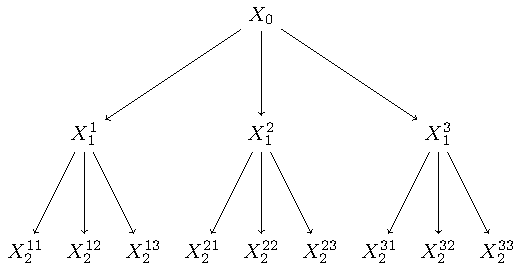
\includegraphics[width=\textwidth]{exponential_tree}
    \caption{Дерево состояний актива}
    \label{fig:tree}
\end{figure}

Рассмотрим оценку сверху \eqref{eq:upper} на небольшом примере: $b = 3, m = 3$. Обозначим операцию + как $\odot$ и $\max$ как $\oplus$. Будем также считать, что дерево состояний актива уже смоделировано и обозначим $h_i\left(X_i^{j_1\cdots j_i}\right) = h_{j_1\cdots j_1}$. Тогда

$$
\begin{aligned}
\Vhat_1 = h_0 &\oplus \left(\frac{h_1}{3}\odot\frac{h_2}{3}\odot\frac{h_3}{3}\right)\oplus \\
    &\oplus \left(\frac{h_1}{3}\odot\frac{h_2}{3}\odot\left(\frac{h_{31}}{9}\odot\frac{h_{32}}{9}\odot\frac{h_{33}}{9}\right)\right) \oplus \\
    &\oplus \left(\frac{h_1}{3}\odot\left(\frac{h_{21}}{9}\odot\frac{h_{22}}{9}\odot\frac{h_{23}}{9}\right)\odot\frac{h_3}{3}\right) \oplus \\
    &\oplus \left(\left(\frac{h_{11}}{9}\odot\frac{h_{12}}{9}\odot\frac{h_{13}}{9}\right)\odot\frac{h_2}{3}\odot\frac{h_3}{3}\right)\oplus \\
    &\oplus\left(\left(\frac{h_{11}}{9}\odot\frac{h_{12}}{9}\odot\frac{h_{13}}{9}\right)\odot\left(\frac{h_{21}}{9}\odot\frac{h_{22}}{9}\odot\frac{h_{23}}{9}\right)\odot\frac{h_3}{3}\right)\oplus \\
    &\oplus \left(\frac{h_1}{3}\odot\left(\frac{h_{21}}{9}\odot\frac{h_{22}}{9}\odot\frac{h_{23}}{9}\right)\odot\left(\frac{h_{31}}{9}\odot\frac{h_{32}}{9}\odot\frac{h_{33}}{9}\right)\right) \oplus \\
    &\oplus \left(\left(\frac{h_{11}}{9}\odot\frac{h_{12}}{9}\odot\frac{h_{13}}{9}\right)\odot\frac{h_2}{3}\odot\left(\frac{h_{31}}{9}\odot\frac{h_{32}}{9}\odot\frac{h_{33}}{9}\right)\right)\oplus \\
    &\oplus \left(\left(\frac{h_{11}}{9}\odot\frac{h_{12}}{9}\odot\frac{h_{13}}{9}\right)\odot\left(\frac{h_{21}}{9}\odot\frac{h_{22}}{9}\odot\frac{h_{23}}{9}\right)\odot\left(\frac{h_{31}}{9}\odot\frac{h_{32}}{9}\odot\frac{h_{33}}{9}\right)\right).
\end{aligned}
$$


В общем виде это выражение выглядит так: $$\Vhat_0 = \oplus_{\gamma\in\Gamma}A\left(\gamma\right),$$ где $\Gamma$ --- полное дерево глубины $m$, т.е. дерево, у всех вершин которого, находящихся на меньшем, чем $m$, расстоянии от корня, есть ровно $b$ дочерних вершин, а у вершин на расстоянии $m$ детей нет, $\gamma$ --- поддерево $\Gamma$, у каждой вершины которого либо 0, либо $b$ дочерних (примеры таких деревьев можно увидеть на рис.~\ref{fig:subtrees}), 
\[A\left(\gamma\right) = \odot_{X\in\gamma} \frac{h_j\left(X\right)}{b^j},\] 
где $j$ --- расстояние от вершины $X$ до корня.


\begin{figure}[!t]
    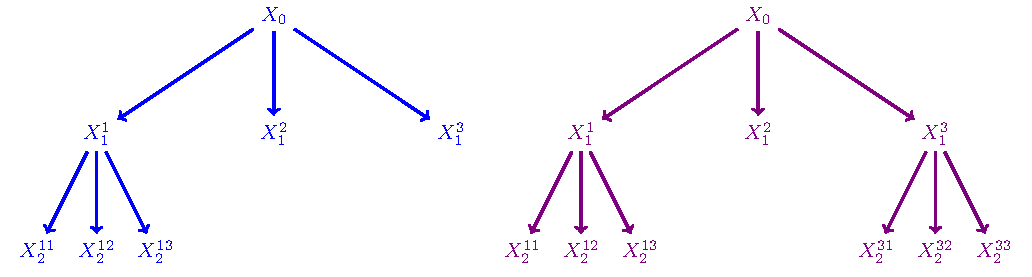
\includegraphics[width=\textwidth]{exponential_subtrees}
    \caption{Примеры поддеревьев $\gamma$}
    \label{fig:subtrees}
\end{figure}

Таким образом, мы получаем выражение для верхней оценки опциона, построенное по отдельным поддеревьям $\gamma\in\Gamma$. Если мы докажем, что для получения состоятельной оценки максимума по всем $\gamma$ необязательно подсчитывать $A\left(\gamma\right)$ для всех $\gamma$, мы добьёмся существенного снижения временных затрат.

\chapter{Сравнение с методом стохастической сетки}

Метод стохастической сетки излагается по \cite{Broadie2004} и (неопубликованной) \cite{Kashtanov2015}.

Метод стохастической сетки также предлагает оценки сверху и снизу для решения \eqref{eq:option-recursive}, но принцип построения оценок несколько отличается от рассматриваемых мною оценок по случайному дереву.

Для описания состояния актива в моменты времени $t_1, \ldots, t_m$ задаются плотности распределения случайной величины, характеризующей состояние актива, в зависимости от времени, обозначим их $g_i\left(\cdot\right)$. Для каждого момента $t\in\left\lbrace t_i \right\rbrace_{i=1}^m$ генерируется b точек $X_{t,1}, \ldots, X_{t, b}$ в соответствии с этой плотностью. Оценка сверху по полученной сетке определяется как
\begin{equation}\begin{aligned}
\hat Q_{T, i} &= h_T\left(X_{T, i}\right), \\
\hat Q_{t, i} &= \max\left\lbrace h_t\left(X_{t, i}\right), \frac{1}{b}\sum_{j=1}^b \hat Q_{t+1}\left(X_{t+1, j}\right) w_t\left(X_{t, i}, X_{t+1, j}\right)\right\rbrace,
\end{aligned}\end{equation}

где $w_t\left(X_{t, i}, X_{t+1, j}\right)$ --- вес, сопоставляемый переходу из $X_i$ в $X_j$. $\hat Q_{0, 0}$ является состоятельной и асимптотически несмещённой оценкой сверху для истинной цены опциона при условии, что веса $w_t$ выбраны должным образом. Основная идея, поясняющая выбор весов, заключается в следующем рассуждении:

$$\begin{aligned}
\ev\left(Q_{t+1}\left(X_{t+1}\right)\middle\vert X_t = x\right) &= \int Q_{t+1}\left(u\right) f\left(x, t, u\right) \mathrm du = \\ &= \int Q_{t+1}\left(u\right) \frac{f\left(x, t, u\right)}{g_{t+1}\left(u\right)}g_{t+1}\left(u\right) \mathrm du = \\ &= \ev\left(Q_{t+1}\left(X_{t+1}\right) \frac{f\left(x, t, u\right)}{g_{t+1}\left(u\right)}\right),
\end{aligned}$$

где $f\left(x, t, u\right)$ — переходная плотность, плотность вероятности того, что актив из состояния $x$ в момент $t$ перейдёт в состояние $u$ к моменту $t+1$. Таким образом, веса компенсируют неточность, порождённую моделированием состояний базового актива без учёта траекторий его развития. Для оценок по случайным деревьям эти веса не нужны, так как плотность распределения $\left.X_{k+1}^{j_1\cdots j_{k+1}}\middle\vert X_{k}^{j_1\cdots j_{k}} = x\right.$ всегда учитывает траекторию, по которой актив попадает в состояние $X_{k+1}^{j_1\cdots j_{k+1}}$ наличием условия в правой части. Следовательно, ряд проблем, вызываемых поиском подходящей плотности $g$ и весов $w$, которые бы обеспечили отсутствие экспоненциального роста дисперсии (решение этой проблемы и предлагается в \cite{Kashtanov2015}), пропадает сам собой.

Для более детального анализа оценка по методу стохастической сетки с учётом поправок, предложенных в \cite{Kashtanov2015}, была реализована. Состояние актива моделировалось лог-нормальным процессом без скачков, в качестве функций плотности на сетке (mesh density functions) были выбраны маргинальные плотности лог-нормального распределения. Веса в оценках были посчитаны с учётом поправок, предложенных в  \cite{Kashtanov2015}. Разберём пример подробнее.

Мы будем считать стоимость опциона колл на один актив. Состояние актива можно промоделировать с помощью геометрического Броуновского движения, то есть $$\mathrm d S_t = S_t\left((r - \delta)\mathrm dt + \sigma \mathrm d Z_t\right),$$ где $S_t$ --- цена актива в текущий момент времени, $Z_t$ --- стандартное Броуновское движение, $r = 3\%$ --- безрисковая процентная ставка, $\delta$ --- дивидендная ставка, $\sigma$ --- волатильность актива. Функция выплат опциона колл на единственный актив определяется как $h_t\left(S_t\right) = \left(S_t - K\right)^+ = \max\left\lbrace S_t - K, 0\right\rbrace$, где $K$ --- цена страйк. Промежуток времени --- $\left[0;1\right]$, в котором исполнение опциона доступно на каждом шаге $i / n, i\in 1:n$. При $n\to\infty$ оценка цены опциона должна приближаться к оценке цены Американского опциона с теми же параметрами.

Для подсчётов понадобятся маргинальные и переходные плотности геометрического Броуновского движения ($S_t \sim GBM\left(r - \delta, \sigma^2\right)$). Для краткости будем называть $\mu = r - \delta$ коэффициентом сноса. Посчитаем переходную плотность:

\begin{align*}
    p_{s, t}\left(x, y\right) &= \frac{\mathrm d}{\mathrm dy} \prob{S_t < y \middle\vert S_s = x} = \\ 
    &= \frac{\mathrm d}{\mathrm dy} \prob{x\cdot\exp\left(\left(\mu - \frac{\sigma^2}{2}\right)\left(t - s\right) + \sigma\underbrace{\xi}_{\sim\mathcal N\left(0, t - s\right)}\right) < y} =  \\ 
    &= \frac{\mathrm d}{\mathrm dy} \prob{\left(\mu - \frac{\sigma^2}{2}\right)\left(t - s\right) + \sigma\xi < \log y - \log x} = \\ 
    &= \frac{\mathrm d}{\mathrm dy} \prob{\sigma\xi < {\log y - \log x - \left(\mu - \frac{\sigma^2}{2}\right)\left(t - s\right)}} = \\ 
    &= p_{\mathcal N\left(0, \sigma^2\left(t - s\right)\right)}\left(\log y - \log x - \left(\mu - \frac{\sigma^2}{2}\right)\left(t - s\right)\right)\cdot \frac{1}{y} = \\
    &= \frac{1}{\sqrt{2\pi\sigma^2\left(t - s\right)}y}\exp\left(-\frac{\log y - \log x - \left(\mu - \frac{\sigma^2}{2}\right)\left(t - s\right)}{2\sigma^2\left(t-s\right)}\right).
\end{align*}

Аналогично выписывается и маргинальная плотность:

$$g_t\left(x\right) = \frac{1}{\sqrt{2\pi}x\sigma\sqrt{t}}\exp\left(-\frac{\log x - \log S_0 - \left(\mu - \frac{\sigma^2}{2}\right)t}{2\sigma^2t}\right).$$

Из-за того, что $g_t$ является плотностью лог-нормального распределения, мы можем моделировать состояния актива на сетке, используя моделирование нормального распределения: $\forall i \in 1\mathbin : M, t\: X_{t, i} = S_0\cdot\exp\left(\left(\mu-\frac{\sigma^2}{2}\right)t + \sqrt t \xi\right), \xi\sim\mathcal N\left(0, \sigma^2\right)$. 

Имея $g_t$ и $p_{s, t}$, можно определить $\rho_{t+1}\left(x, j\right) = p_{t, t+1}\left(x, X_{t+1, j}\right) / g_{t+1}\left(X_{t+1, j}\right)$ и выписать в явном виде оценки по сетке:

\[\begin{aligned}
\hat Q _{T, i} &= h_T\left( X_{T, i}\right), \\
\hat Q _{t, i} &= \max\left\lbrace h_t\left( X_{T, i}\right), \frac{\sum_{j=1}^M \rho_{t+1}\left(x, j\right) \hat Q_{t+1, j}}{\sum_{j=1}^M \rho_{t+1}\left(x, j\right)}\right\rbrace.\end{aligned}\]

\begin{figure}[t!]
    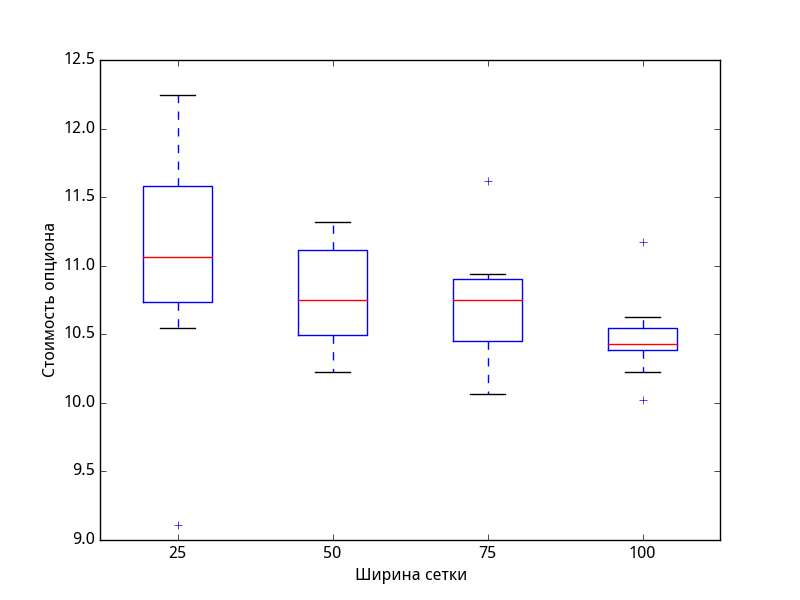
\includegraphics[width=\textwidth]{plot_100}
    \caption{Оценки по сетке стоимости опциона при $n = 50$ моментах исполнения}
    \label{fig:boxplot}
    $r = 3\%, \delta = 10\%, \sigma = 30\%$. Начальная цена актива $S_0$ и цена страйк $K$ одинаковы и равны 100.
\end{figure}

Результаты моделирования представлены на рис.~\ref{fig:boxplot}. Как и предполагалось, оценка уточняется по мере увеличения ширины сетки. Аналогичные результаты получаются и для других $n$.

\conclusion
Получена формулировка задачи как задачи поиска максимума по всем возможным поддеревьям. Такая формулировка позволяет рассчитывать на то, что при применении соответствующих теорем  мы получим состоятельную оценку с меньшими временными затратами, чем в изначальном методе.
В дальнейшем планируется разработать такую состоятельную оценку.

Рассмотрена и реализована оценка стоимости опциона по стохастической сетке, которая  обладает меньшей вычислительной сложностью.
\bibliographystyle{ugost2008}
\bibliography{../biblio-u}

\end{document}